\documentclass[a4paper,twoside]{article}

\usepackage{blindtext}
\usepackage{geometry}

% Chinese support
\usepackage[UTF8, scheme = plain]{ctex}

% Page margin layout
\geometry{left=2.3cm,right=2cm,top=2.5cm,bottom=2.0cm}

\usepackage{listings}
\usepackage{xcolor}
\usepackage{geometry}
\usepackage{amsmath}
\usepackage{float}
\usepackage{hyperref}

\usepackage{graphics}
\usepackage{graphicx}
\usepackage{subfigure}
\usepackage{epsfig}
\usepackage{float}
\usepackage{algorithm}
\usepackage[noend]{algpseudocode}

\usepackage{booktabs}
\usepackage{threeparttable}
\usepackage{longtable}
\usepackage{listings}
\usepackage{tikz}
\usepackage{multicol}

% cite package, to clean up citations in the main text. Do not remove.
\usepackage{cite}

\usepackage{color,xcolor}

%% The amssymb package provides various useful mathematical symbols
\usepackage{amssymb}
%% The amsthm package provides extended theorem environments
\usepackage{amsthm}
\usepackage{amsfonts}
\usepackage{enumerate}
\usepackage{enumitem}
\usepackage{listings}

\usepackage{indentfirst}
\setlength{\parindent}{2em} % Make two letter space in the first paragraph
\usepackage{setspace}
\linespread{1.5} % Line spacing setting
\usepackage{siunitx}
\setlength{\parskip}{0.5em} % Paragraph spacing setting

\renewcommand{\figurename}{图片}
\renewcommand{\lstlistingname}{代码} 
\renewcommand{\tablename}{表格}
\renewcommand{\contentsname}{目录}
\renewcommand\refname{参考文献}
\graphicspath{ {img/} }
\newcommand{\upcite}[1]{\textsuperscript{\textsuperscript{\cite{#1}}}}



%%%%%%%%%%%%%
\newcommand{\StudentNumber}{22920202200764}  % Fill your student number here
\newcommand{\StudentName}{刘本宸}  % Replace your name here
\newcommand{\PaperTitle}{智能小车实验报告}  % Change your paper title here
\newcommand{\PaperType}{学科实践(一):智能机器人理论与实践} % Replace the type of your report here
\newcommand{\Date}{2023年02月27日}
\newcommand{\College}{厦门大学 信息学院}
\newcommand{\Class}{人工智能二班}
\newcommand{\CourseName}{学科实践(一):智能机器人理论与实践}
%%%%%%%%%%%%%

%% Page header and footer setting
\usepackage{fancyhdr}
\usepackage{lastpage}
\pagestyle{fancy}
\fancyhf{}
% This requires the document to be twoside
\fancyhead[LO]{\texttt{\StudentName }}
\fancyhead[LE]{\texttt{\StudentNumber}}
\fancyhead[C]{\texttt{\PaperTitle }}
\fancyhead[R]{\texttt{Page {\thepage},Total \pageref*{LastPage}}}

\title{\PaperTitle}
\author{\StudentName}
\date{\Date}


\lstset{
	basicstyle          =   \sffamily,          % 基本代码风格
	keywordstyle        =   \bfseries,          % 关键字风格
	commentstyle        =   \rmfamily\itshape,  % 注释的风格,斜体
	stringstyle         =   \ttfamily,  % 字符串风格
	flexiblecolumns,                % 别问为什么,加上这个
	numbers             =   left,   % 行号的位置在左边
	showspaces          =   false,  % 是否显示空格,显示了有点乱,所以不现实了
	numberstyle         =   \zihao{-5}\ttfamily,    % 行号的样式,小五号,tt等宽字体
	showstringspaces    =   false,
	captionpos          =   t,      % 这段代码的名字所呈现的位置,t指的是top上面
	frame               =   lrtb,   % 显示边框
}

\lstdefinestyle{PythonStyle}{
	language        =   Python, % 语言选Python
	basicstyle      =   \zihao{-5}\ttfamily,
	numberstyle     =   \zihao{-5}\ttfamily,
	keywordstyle    =   \color{blue},
	keywordstyle    =   [2] \color{teal},
	stringstyle     =   \color{magenta},
	commentstyle    =   \color{red}\ttfamily,
	breaklines      =   true,   % 自动换行,建议不要写太长的行
	columns         =   fixed,  % 如果不加这一句,字间距就不固定,很丑,必须加
	basewidth       =   0.5em,
}

\lstdefinestyle{CppStyle}{
	language        =   c++,
	basicstyle      =   \zihao{-5}\ttfamily,
	numberstyle     =   \zihao{-5}\ttfamily,
	keywordstyle    =   \color{blue},
	keywordstyle    =   [2] \color{teal},
	stringstyle     =   \color{magenta},
	commentstyle    =   \color{red}\ttfamily,
	breaklines      =   true,   % 自动换行,建议不要写太长的行
	columns         =   fixed,  % 如果不加这一句,字间距就不固定,很丑,必须加
	basewidth       =   0.5em,
}

\algnewcommand\algorithmicinput{\textbf{输入}}
\algnewcommand\algorithmicoutput{\textbf{输出}}
\algnewcommand\Input{\item[\algorithmicinput]}%
\algnewcommand\Output{\item[\algorithmicoutput]}%

\usetikzlibrary{positioning, shapes.geometric}


\begin{document}

\makeatletter % change default title style
\renewcommand*\maketitle{%
	\begin{center}
		\bfseries  % title 
		{\LARGE \@title \par}  % LARGE typesetting
		\vskip 1em  %  margin 1em
			{\global\let\author\@empty}  % no author information
			{\global\let\date\@empty}  % no date
		\thispagestyle{empty}   %  empty page style
	\end{center}%
	\setcounter{footnote}{0}%
}
\makeatother

\thispagestyle{empty}

\vspace*{1cm}

\begin{figure}[h]
	\centering
	
\includegraphics[width=4.0cm]{logo.png}
\end{figure}

\vspace*{1cm}

\begin{center}
	\Huge{\textbf{\PaperType}}

	\Large{\PaperTitle}
\end{center}

\begin{table}[h]
	\centering
	\begin{Large}
		\renewcommand{\arraystretch}{1.5}
		\begin{tabular}{p{3cm} p{5cm}<{\centering}}
			姓 \quad 名 & \StudentName (第一组) \\
			\hline
			学 \quad 号 & \StudentNumber        \\
			\hline
			日 \quad 期 & \Date                 \\
			\hline
			学 \quad 院 & \College              \\
			\hline
			班 \quad 级 & \Class                \\
			\hline
			课 \quad 程 & \CourseName           \\
			\hline
		\end{tabular}
	\end{Large}
\end{table}
\newpage
% 目录
\tableofcontents
\newpage


\section{选题以及选题依据}
在课程的开始,我们先认识了ROS2系统和给定的小车的一些基本模块,后面我们开始循着老师给的选题进行实践。
选题实现了两个项目。这两个项目的关系是递进的。
第一个项目是基于小车的智能巡线,另外一个是基于SLAM、视觉系统以及抓取的自动寻物小车。

ROS(Robot Operating System)是我们本次机器人实践的软件平台。它提供一系列程序库和工具以帮助软件开发者创建机器人应用软件。
它提供了硬件抽象、设备驱动、库函数、可视化、消息传递和软件包管理等诸多功能。ROS 遵守 BSD 开源许可协议,是开源的机器人控制框架。
我们使用的ROS2是ROS的升级版本,ROS2引入了数据分发服务通信协议,各个软硬件模块通过节点进行通信,而且减少了框架的内存使用。
同时基于ROS2系统,我们还可以利用自带的Rviz等程序进行小车的状态可视化,这大大方便了我们的学习。
并且我们使用的ROS2有对应的开源社区 \footnote{ http://www.ros.org/ \quad http://wiki.ros.org/} ,在开源社区内已经有了一部分成熟,易用,鲁棒性强的“轮子”供我们学习和调用。
同时我也通过Github, Youtube等多个网站上搜集了相关资料进行学习和吸收,这些学习资料也帮助了我快速完成后面的任务。

\begin{figure}[htbp]
	\centering
	\begin{minipage}{0.49\linewidth}
		\centering
		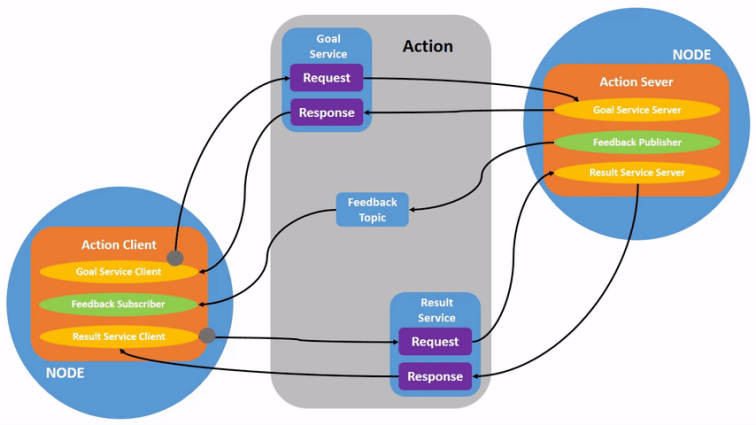
\includegraphics[width=0.75\linewidth]{ros2character.png}
		\caption{ROS2通信方式}
		\label{chutian1}%文中引用该图片代号
	\end{minipage}
	%\qquad
	\begin{minipage}{0.49\linewidth}
		\centering
		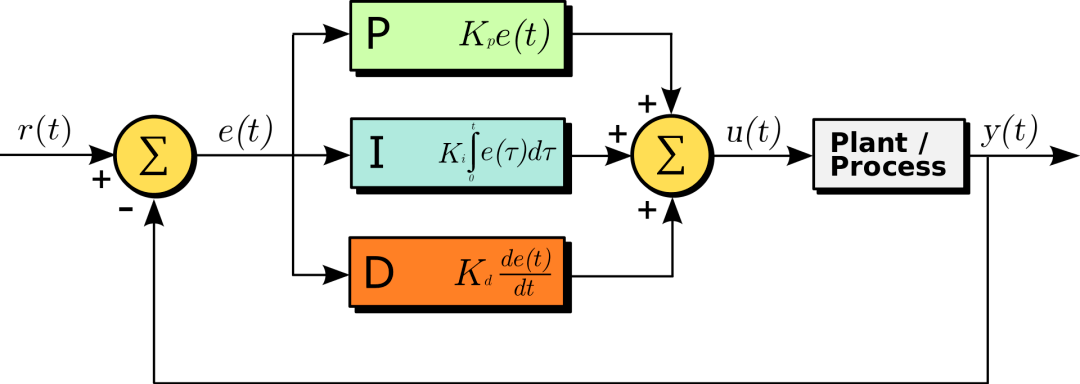
\includegraphics[width=0.9\linewidth]{pidalgorithm.png}
		\caption{PID控制算法}
		\label{chutian2}%文中引用该图片代号
	\end{minipage}
\end{figure}



小车智能巡线主要是实现一个可以根据小车前部的视觉输入,自动研判当前位置,自动进行车轮速度调节和转向,并且
判断是否达到了寻迹终点,到达终点时自动停止关闭相关服务,终止相关进程。在实践寻迹小车之前我们已经进行了小车
基本模块的认识,而且还组内阅读,讨论了相关代码。在老师给定的代码框架之下,我们进行了部署,在小车上进行了测试。
整体上是一次项目的练兵,从框架设计,到功能和逻辑的拆分,到代码实现,再到部署。整个流程我们小组完整的走了一遍。
在这次学习和实现巡线小车的时候,我们还学习了PID算法。PID算法是工业应用中最广泛算法之一,
也是一种非常古老的算法(有一百多年的历史了),在对系统的控制中,可自动对控制系统进行准确且迅速的校正。
在我们的小车实践里面我们使用了PID算法,巧妙的处理了给定地图中比较“大”的转弯,这样,在转弯时,我们的小车的前摄像头不会
跟丢贴在地板上的“实线”,出现站在拐弯处原地不动的情况。

自动寻物小车是在自动巡线小车的升级版。在已有的控制算法基础上,我们在实现小车最终的功能时,尝试综合使用了小车上已有的多个模块,
比如:激光雷达,摄像头模块,机械臂上的驱动模块以及机械臂上的视觉模块。
而且在软件上面,我们基于已有的硬件模块进行了多个小车功能节点的编写,比如:位姿位置定位模块,物体识别模块,驱动模块,抓取模块,巡航模块等等。
我们通过激光模块对整个地图进行建模,方便小车在地图中定位自己以及规划路径。
并且我们尝试了训练一个tiny-YOLOv3的神经网络用于进行物体的识别。这个神经网络不仅在巡航时给出了物体相对于车的位置,为车靠近物体提供了方向,
而且还给出了物体相对于机械臂的位置,这个对于后面机械臂抓取物体方面有很大的帮助。
在完成抓取任务之后,小车会在我们的设定之下完成“回家操作”,这一步也是基于地图和导航的。
自此,小车的各个部分相互关联工作,形成了我组的自动寻物小车。



\newpage
\section{小组分工和工作计划表}
\subsection{小组分工}
\begin{itemize}
	\item 刘本宸(组长) \quad
	      负责整个组的统筹工作,代码框架设计、代码具体实现、部署和优化,保证可以完成课程选题以及整体论文撰写。
	\item 孟 \quad 媛\quad
	      负责制作物体训练集,完成PPT报告的制作
	\item 姜小康 \quad
	      负责后勤工作,解决小车硬件故障,小车充电等
	\item 刘宇菲 \quad 训练tiny-YOLOv3神经网络,生成权重文件,部署神经网络
	\item 贾惠卿 \quad 负责管理和维护小车机械臂,保证机械臂基本功能正常
\end{itemize}
\subsection{工作计划}
\begin{itemize}
	\item 1-4周 \quad 熟悉ROS2机器人操作系统,熟练控制机器人,对各个小模块进行编程和功能测试
	\item 5-6周 \quad 编程实现巡线功能,并且实现参数的调优,并且记录相关参数
	\item 7-8周 \quad 编程实现寻找、抓取功能,优化程序运行流程
\end{itemize}
\newpage
\section{实验过程}
\subsection{硬件模块}
机器人整体外观如下图所示,框架采用钣金作为支撑件,在底盘上有四个电机在机器人的左边配备有肩屏,
在正上方后部是机器人的中央处理器和机械臂控制模块,
在正上方的前部是机械臂模块。最前面是G4激光雷达与奥比中光大白相机。
还有一个遥控器但是并没有在图中给出。
\begin{figure}[htbp]
	\begin{center}
		\includegraphics*[width=0.9\linewidth]{robothardware.png}
		\caption{小车基本外观}
	\end{center}
\end{figure}
\paragraph{机器人机械部分}
\textbf{SCOUT MINI 智能移动底盘}是四轮驱动的,性能优越。该底盘在尾部增加了充电接口,
而且在后部还有扩展接口,交互模块,供电模块等等。足以成为其他模块的底座。
处理器采用的是英伟达的\textbf{Nvidia Jetson Nano小型计算机},据英伟达的描述,该计算机
专为支持入门级边缘AI应用程序和设备而设计。但是在实际应用中我发现
这个小型计算机的性能并没有那么强劲,需要程序员亲自进行资源分配,而且要在程序设计时做好容灾处理。
机械臂是配备的\textbf{Alpha机械臂}整体外形紧凑,安装便捷。PC端提供了BrobotStudio集成软件,
该软件融合了鼠标控制、图形化编程等多种功能,并提供了多种控制机械臂的运动形式,而且它支持多种编程语言,
方便我们使用Python3和ROS2框架进行编程控制。

\begin{figure}[htbp]
	\centering
	\begin{minipage}{0.49\linewidth}
		\centering
		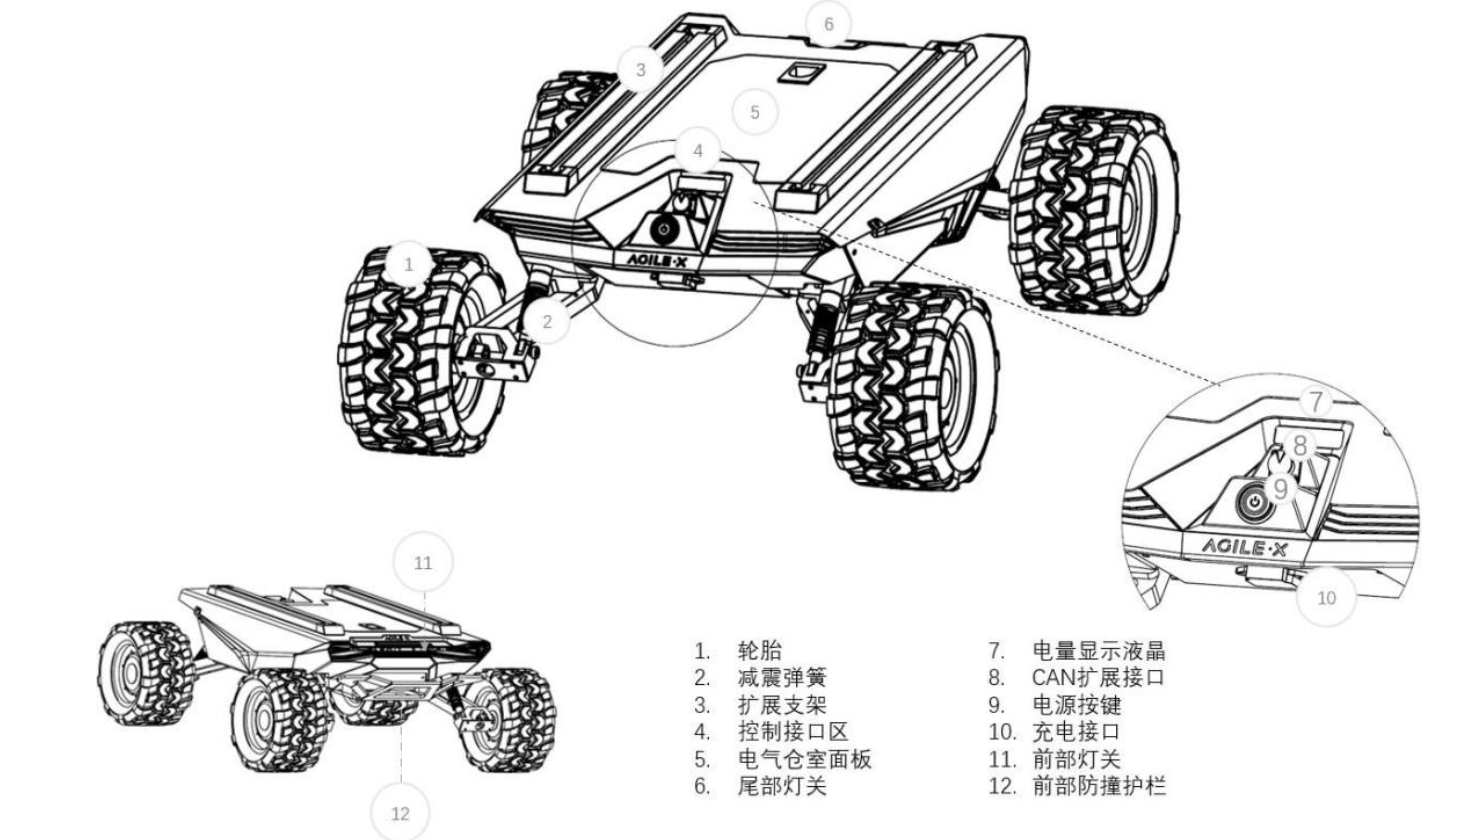
\includegraphics[width=1.0\linewidth]{scoutmini.png}
		\caption{Scout Mini 底盘}
	\end{minipage}
	%\qquad
	\begin{minipage}{0.49\linewidth}
		\centering
		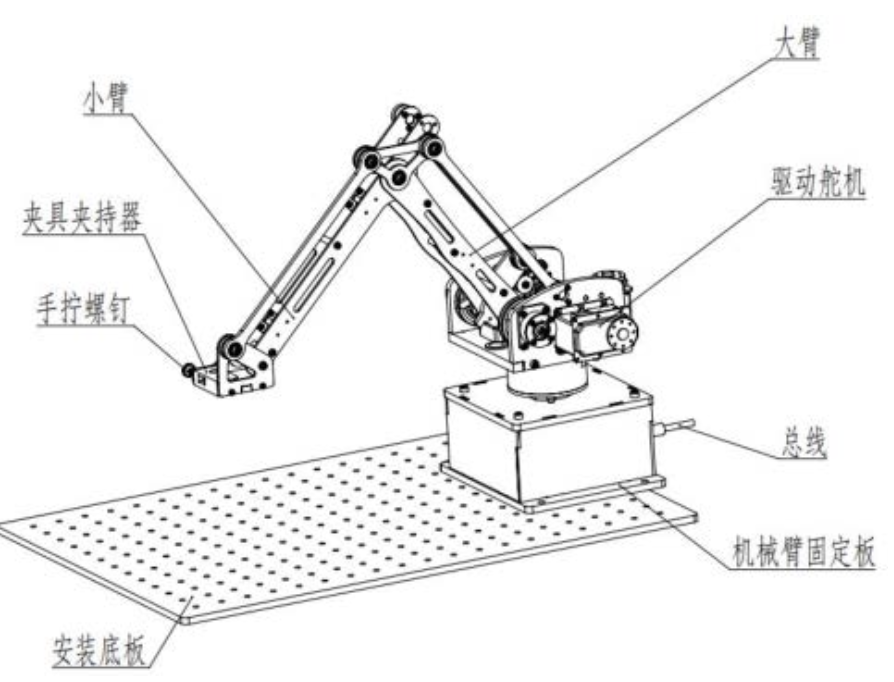
\includegraphics[width=0.9\linewidth]{alpha.png}
		\caption{Alpla机械臂}
	\end{minipage}
\end{figure}
\newpage
\paragraph{机器人传感部分}
\textbf{ORBBEC®Dabai 相机}是基于双目结构光3D成像技术的深度相机,有左右红外相机,可以
计算物体对应深度,而且还有基本的图像接收功能。
\textbf{YDLIDAR G4 激光雷达}是基于三角测距原理的一款激光雷达。不仅可以测距,并且在测距的同时
,机械结构360度旋转,不断获取角度信息,从而实现了360度扫描测距,输出扫描环境的点云数据,这个
点云数据可以帮助我们小车构建地图,获取小车位置。而且摄像头信息还可以通过Rviz进行可视化。
\textbf{摄像头 (附于Alpha机械臂上)}这个摄像头主要是在抓取的时候可以获取物体的和机械臂的相对位置,
在抓取的时候可以准确定位,并且进行抓取,这个摄像头依附于机械臂夹具之上,故图片不再给出。
\begin{figure}[htbp]
	\begin{center}
		\includegraphics*[width=0.7\linewidth]{sensors.png}
		\caption{基本传感器}
	\end{center}
\end{figure}
\paragraph{机器人遥控部分}
遥控主要是使用遥控器,是随着机器人配备的。在对应的SWB模式置为ON就可以实现
遥控器对于小车底盘控制,反之则由机器人上面的程序进行运动控制。小车的油门是在左手边,
类似我们小时候玩的遥控汽车。
\begin{figure}[htbp]
	\begin{center}
		\includegraphics*[width=0.7\linewidth]{controller.png}
		\caption{遥控器}
	\end{center}
\end{figure}
\newpage
\subsection{软件模块}
\paragraph*{Ubuntu}
Ubuntu是一个linux的发行版,是一个被广泛应用的操作系统,它基于UNIX框架,所以对硬件操作这种底层的开发工作
比较友好。我们使用的是Ubuntu20.04,还带有桌面图形化操作。

\paragraph*{ROS2}
ROS2是一个迭代升级过的机器人操作系统,它支持多种操作系统(Linux, MacOS, Windows等等),而且
改善了对Python3的支持,这降低了我们的编程难度,提高了兼容性。而且在ROS2中,节点之间使用一种称
为“Discovery”的发现机制来帮助彼此建立连接。这样的节点通讯机制可以减少内存,处理器等系统资源的消耗。
并且有许多已有的“轮子”供我们使用。我们使用的是ROS2 Melodic版本。

\paragraph*{Rviz}
Rviz是ROS中一款三维可视化平台,一方面能够实现对外部信息的图形化显示,另外还可以通过rviz给对象发布控制信息,从而实现对机器人的监测与控制。
在我们的实验中,我们使用Rviz进行了小车的建图、位姿调整、巡航的可视化。而且在Rviz中还可以实时显示我们小车前方摄像头的画面。
有利于我们后期对小车进行调试。

\begin{figure}[htbp]
	\centering
	\begin{minipage}{0.49\linewidth}
		\centering
		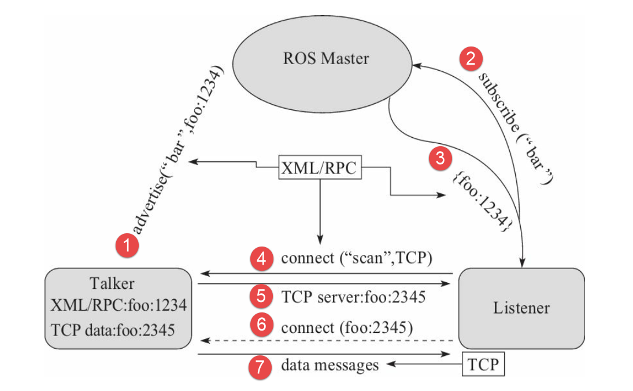
\includegraphics[width=1.0\linewidth]{rosframework.png}
		\caption{ROS2 框架}
	\end{minipage}
	%\qquad
	\begin{minipage}{0.49\linewidth}
		\centering
		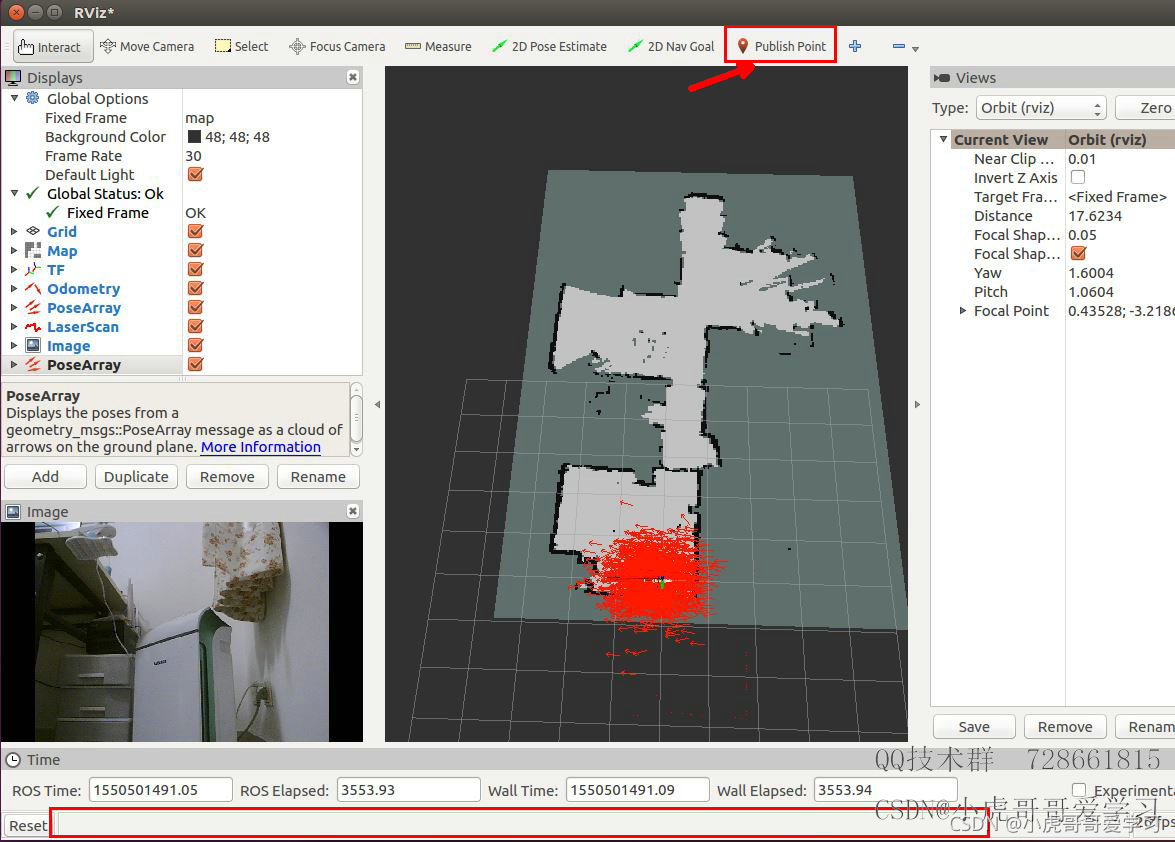
\includegraphics[width=0.9\linewidth]{rviz.png}
		\caption{Rviz可视化(图源自网络)\upcite{rvizvisual}}
	\end{minipage}
\end{figure}


\subsection{设计技术参数}
\begin{enumerate}
	\item 巡线实验
	      \begin{itemize}
		      \item 颜色过滤参数:Upper = (73,43,46) Lower = (124,255,255) (为HSV颜色)
		      \item $K_p = .18$ ,$K_i = .004$,$K_d = .0001$ (参数解释在下面公式解读会提到)
	      \end{itemize}
	\item 寻物实验
	      \begin{itemize}
		      \item 巡航节点速度信息:  max\_vel\_x: 0.50
		            min\_vel\_x: 0
		            acc\_lim\_x: 1.0
		      \item 小熊颜色过滤参数:Upper = (35, 180, 190), Lower = (10, 80, 80) 为HSV颜色
		      \item 小车碰撞容忍度:xy\_goal\_tolerance: 0.5 \quad yaw\_goal\_tolerance: 0.5
		      \item 巡航节点坐标列表:

		            [
		            (-3.44, -0.78, 0.0, -125.3),
		            (-3.73, -4.81, 0.0, -125.5),
		            (-6.47, -2.32, 0.0, 151.2),


		            (-8.59, -5.44, 0.0, -122.67),
		            (-5.43, -3.74, 0.0, 28),
		            (-7.41, -6.63, 0.0, -135.16),


		            (-5.72, -7.78, 0.0, -33.56),
		            (-1.97, -2.31, 0.0, 53.65),
		            (-5.03, -1.08, 0.0, 173.53),


		            (-2.76, -0.78, 0.0, 52.78),
		            (-3.04, 2.49, 0.0, 96),
		            ]

		            四元组分别为\textbf{(x, y, z, Orientation)}
		      \item Yolov3-tiny权重文件:同级列表中有权重文件,名为:yolov3-tiny-Vision-bear-2000.weights
	      \end{itemize}
\end{enumerate}
\subsection{程序架构以及实现思路}
\paragraph{巡线实验--Task1}
第一个巡线实验主要是需要协调好运动模块和视觉模块。首先视觉模块需要持续接受信号,并且将信号转化
为对应的二值化图像,即把线从背景中分离开来,让最后的图像中只有线,之后通过计算对应的线的视觉中心,
通过计算视觉中心的偏移和PID算法来把视觉信号转化为运动信号和转向信号。最后将运动信号输出到底盘上。
当没有线的输入信号的时候,机器就判断已经走到终点,程序停止。程序框图在附录中 (图片\ref*{task1frame})。

\paragraph*{寻物实验--Task2}
第二个寻物实验会用到多种的传感器。首先要保证地图可以建成,地图的搭建使用的是激光雷达进行建图。建成的图片在
文件附录中可以看到。并且小车需要通过对于点云的扫描来确定自己的位置和朝向。在寻找物体的过程中,小车需要开启导航模块,
需要循着我们既定的路线进行寻址,以保证小车可以遍历地图上所有的点。加之,我们需要一直启动摄像机节点
并且启动物体检测服务,如果在小车的巡航的时候发现了物体,就要进入寻找物体并且抓取的逻辑。而且在抓取逻辑结束之后
需要回到起点,这也是需要导航服务工作的。程序框图在附录中 (图片\ref*{task2frame}).


\newpage
\section{实验结果检测}

\subsection{巡线模块}
巡线模块主要是OpenCV的使用,使用这个视觉库对于输入画面先进行二值化再进行判断。如果路线转弯则向底盘发送转弯信息,否则就是直线行走
如果摄像头丢失了图像的信息,说明已经走到了尽头,开始进入下一个任务(即Task2)。

当然这个地方有一个比较tricky的地方就是,可以对输入画面先进行分割,比如在本次实验中,我们在判断巡线轨迹的时候
只截取了摄像头(480*720)视野内的最下方的60条像素。因为我们看到的“线”大多数都在视野的下半区。这样可以减少二值化的计算次数,
减少性能的浪费。

然后需要在轨迹寻迹的时候加入PID算法判断,使得小车转弯的时候尽量平滑。当然这一部分的参数调节需要自己手动。
后来我发现其实如果要追求较快的速度,也可以在直线的时候使用PID算法,在接受的画面中通过计算直线在画面中的占比
来确定是否可以加速。

适配于巡线小车的PID控制算法公式在下面已经给出,$K_p$是比例增益,$K_i$是积分增益,$K_d$是微分增益,e(t)是我们的小车的偏转状态变量。
其中三个增益量是我们可以调整的参数。在本次实验中,我们经过多次的实验已经在最后调整出了最优的参数。这个参数被适用于我们的巡线模块。

\begin{equation}
	u(t) = K_pe(t)+K_i\int_0^te(\tau)d\tau+K_d\cfrac{de(t)}{dt}
\end{equation}

\subsection{巡航模块}
巡航模块是基于地图和激光雷达的。主要是SLAM(Simultaneous Localization and Mapping,简称SLAM)技术的应用。
一开始我们会开启雷达,并且用遥控器控制机器人遍历一遍整个地图,直到整个地图都被雷达扫描完毕,生成一个数字地图(图片:\ref*{map}).
在我们建立好地图之后,会以我们的开始作为原点建立二维坐标系。并且在建图时还会生成对应的转向角度,这个
角度在后面会用于搭建地图服务,让机器人知道自己在哪个地方。我们用一个三元组\textbf{(X, Y, Orientation)}来描述机器人当前位姿。

\begin{figure}[htbp]
	\begin{center}
		\includegraphics*[width=0.65\linewidth]{map.png}
		\caption{使用激光雷达建模的地图}\label{map}
	\end{center}
\end{figure}
在巡线结束后,机器人进行Global Localization的操作,机器人会启动激光雷达,扫描接收到的激光信号,并且通过AMCL(蒙特卡洛)粒子滤波定位算法
来进行自身的全局重定位,在围绕场地后机器人会将自己的方向向量置为正确的方向。
在此之后,机器人会开始自动按照巡航节点队列依次访问巡航,在巡航过程中如果视觉模块检测到了物体的出现,就会抛弃后面的巡航任务。转而进行抓取、
回到起点的操作。

还有一点要注意就是,机器人在接受到一个目标节点的巡航任务时,会分别调用两个函数global\_planner和local\_planner,这两个函数有一个参数tolerance控制小车在行进的过程中
不会碰撞到墙壁。如果这个小车在巡航的时候靠近墙壁太近的话,会导致小车被墙“卡”住。所以在编程实践时,一方面要注意巡航节点的选取要远离墙壁,
另一方面要在scout\_param中调小tolerance的值,让小车不会离墙过远的时候认为自己遇到了障碍。

\begin{figure}[htbp]
	\centering
	\begin{minipage}{0.49\linewidth}
		\centering
		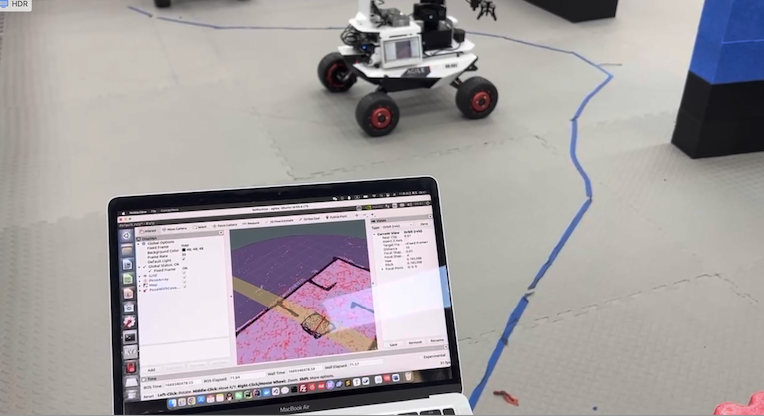
\includegraphics[width=1.0\linewidth]{compassbegin.png}
		\caption{全局重定位开始}
	\end{minipage}
	%\qquad
	\begin{minipage}{0.49\linewidth}
		\centering
		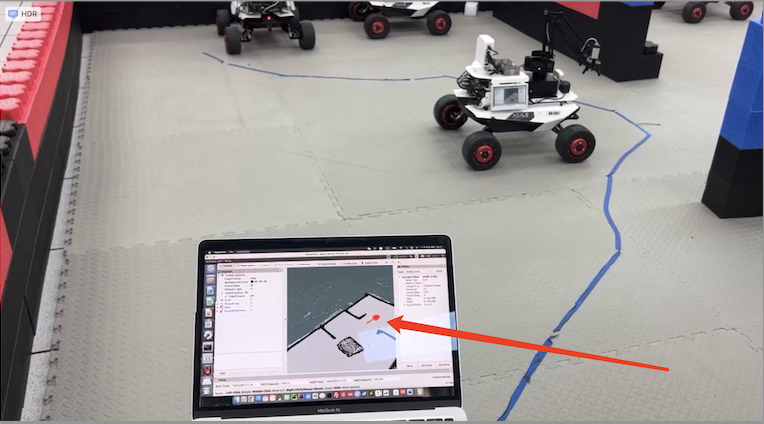
\includegraphics[width=1.0\linewidth]{compassend.png}
		\caption{全局重定位结束}
	\end{minipage}
\end{figure}

\subsection{视觉模块}
视觉模块主要是运用Dabai前置摄像头接收图像后,用我们的订阅节点来订阅机器人所发送出来的图像,并且
使用计算机视觉亦或是深度学习、神经网络的方法对已有图像进行处理,并且提取图像中的信息。
在本次实验中,我们对两种方法都有涉猎。实践证明,深度学习方法识别物体的准确度是相当的高的,但是
深度学习框架是非常耗费资源的; 计算机视觉方法是需要不断调整一些参数,但是计算速度快,节省系统资源
特别在我们这种边缘计算的场景之下,是可以大大提高系统其他进程的运行速度的。当然还有一种对象检测算法可以
应用在这个视觉模块上面,但是这个需要的资源也是相当多的,我们组只是做了相关的尝试并没有在最后任务的实现中
使用这个物体检测模块。
\paragraph{深度学习}
深度学习方法我们是训练了一个属于“物体”自己的神经网络。我们先对小熊进行了视频拍摄,然后将视频每一帧分出来,
并且使用精灵标注助手 \footnote{下载地址: https://www.xiazaiba.com/html/115079.html} 这个标注软件,
制作了一个“小熊”的VOC数据集\upcite{createdataset}。然后我们用Colab\footnote{https://colab.research.google.com}白嫖了一
些计算资源,训练了一个自己的tiny-YOLOv3神经网络\upcite{trainyolo}。
识别效果还是相当好的。下面有识别的效果图,图中的物体识别置信度为\textbf{0.92}。但是有一个问题就是,如果开启了
神经网络对于摄像头图片进行实时识别,那样剩余可用的内存容量会很少,无法开启其他的服务(如地图服务)。

\paragraph{计算机视觉}
这一种图像处理方法主要是使用OpenCV库对小熊的一些颜色特征进行提取。这种方法带有先验知识影响,即小熊是偏黄色的
而我们的迷宫挡板多数都是黑色、蓝色、红色,使用类似图像遮罩的方法可以将小熊的颜色从背景板里面提取出来。
然后我们一旦获取到了小熊对应的颜色信息,而且它的颜色占据了整个摄像头足够大的区域,我们就认为我们的小车已经在
小熊周围了,接下来就会去启动靠近小熊并且抓取的功能。(可惜这部分实验拍摄的图片已经丢失,但是代码还在,会在附录一并给出)


\paragraph{物体检测算法(模板匹配)}
模板匹配主要是使用了SURF、SIFT、ORB、FAST等一系列算法,这一部分算法被适配进了ROS 2开源的库 \footnote{http://wiki.ros.org/find\_object\_2d} 进行物体的特征提取并且进行检测。
我们在给定目标物体的图片的情况下,提取特征点,然后将特征点与视觉传入的物体的特征进行比对。而且这种算法还可以返回物体在图像中的具体位置在用单应性矩阵的变换\upcite{matrix}之后就可以得到物体在摄像头画面中的具体位置了。但是实践证明这种方法也不是特别好,因为基于特征点的匹配对光线的要求特别高,再者如果物体姿态与上一秒采样
的姿势不同,算法就无法正确识别。(可惜这部分实验拍摄的图片已经丢失,但是代码还在,会在附录一并给出)

\begin{figure}[htbp]
	\centering
	\begin{minipage}{0.49\linewidth}
		\centering
		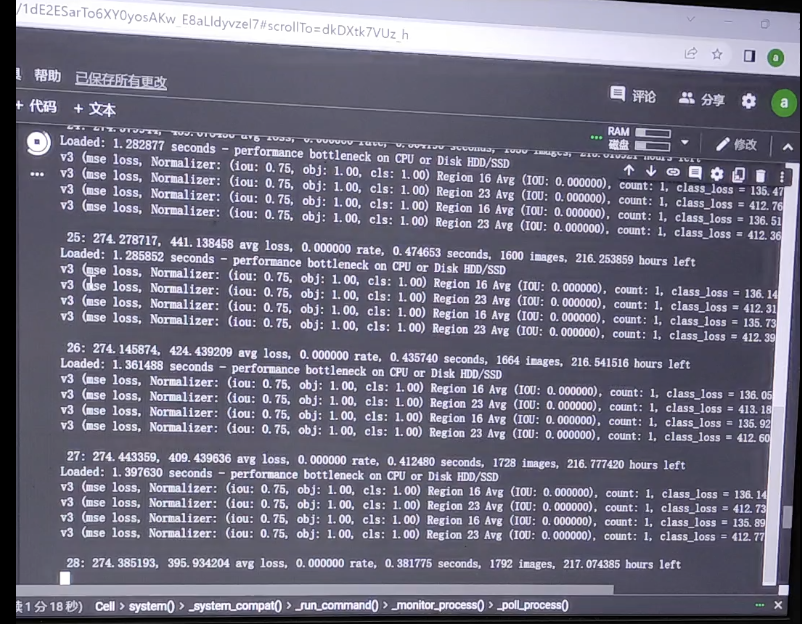
\includegraphics[width=1.0\linewidth]{train.png}
		\caption{使用Colab进行神经网络训练}
	\end{minipage}
	%\qquad
	\begin{minipage}{0.49\linewidth}
		\centering
		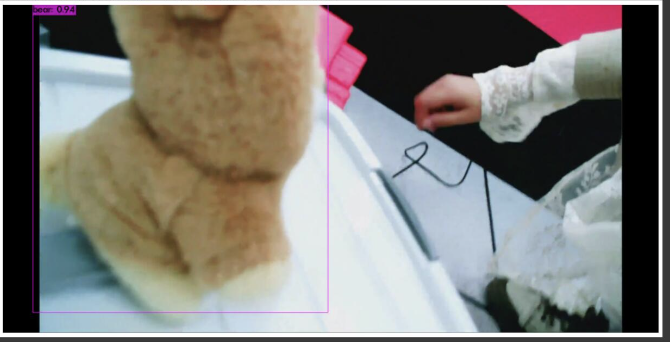
\includegraphics[width=1.0\linewidth]{yoloexample.png}
		\caption{使用新训练的tiny-YOLOv3进行识别}
	\end{minipage}
\end{figure}

\begin{figure}[htbp]
	\centering
	\begin{minipage}{0.49\linewidth}
		\centering
		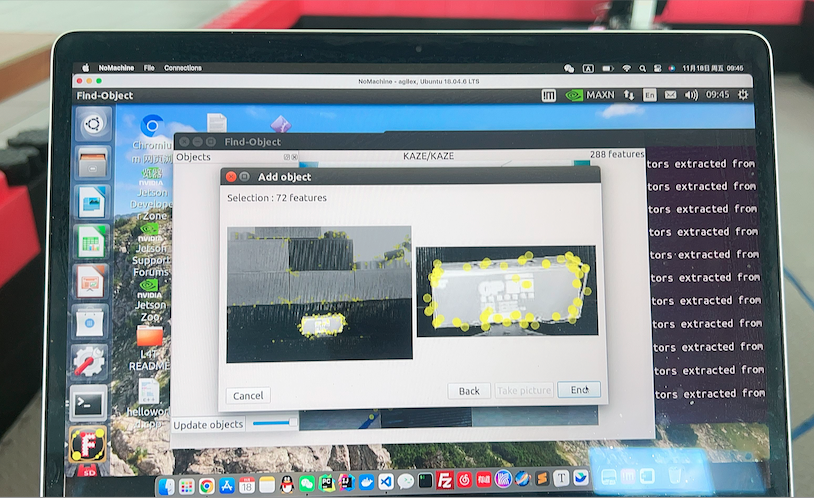
\includegraphics[width=1\linewidth]{findobject.png}
		\caption{模板匹配结果}
	\end{minipage}
	%\qquad
	\begin{minipage}{0.49\linewidth}
		\centering
		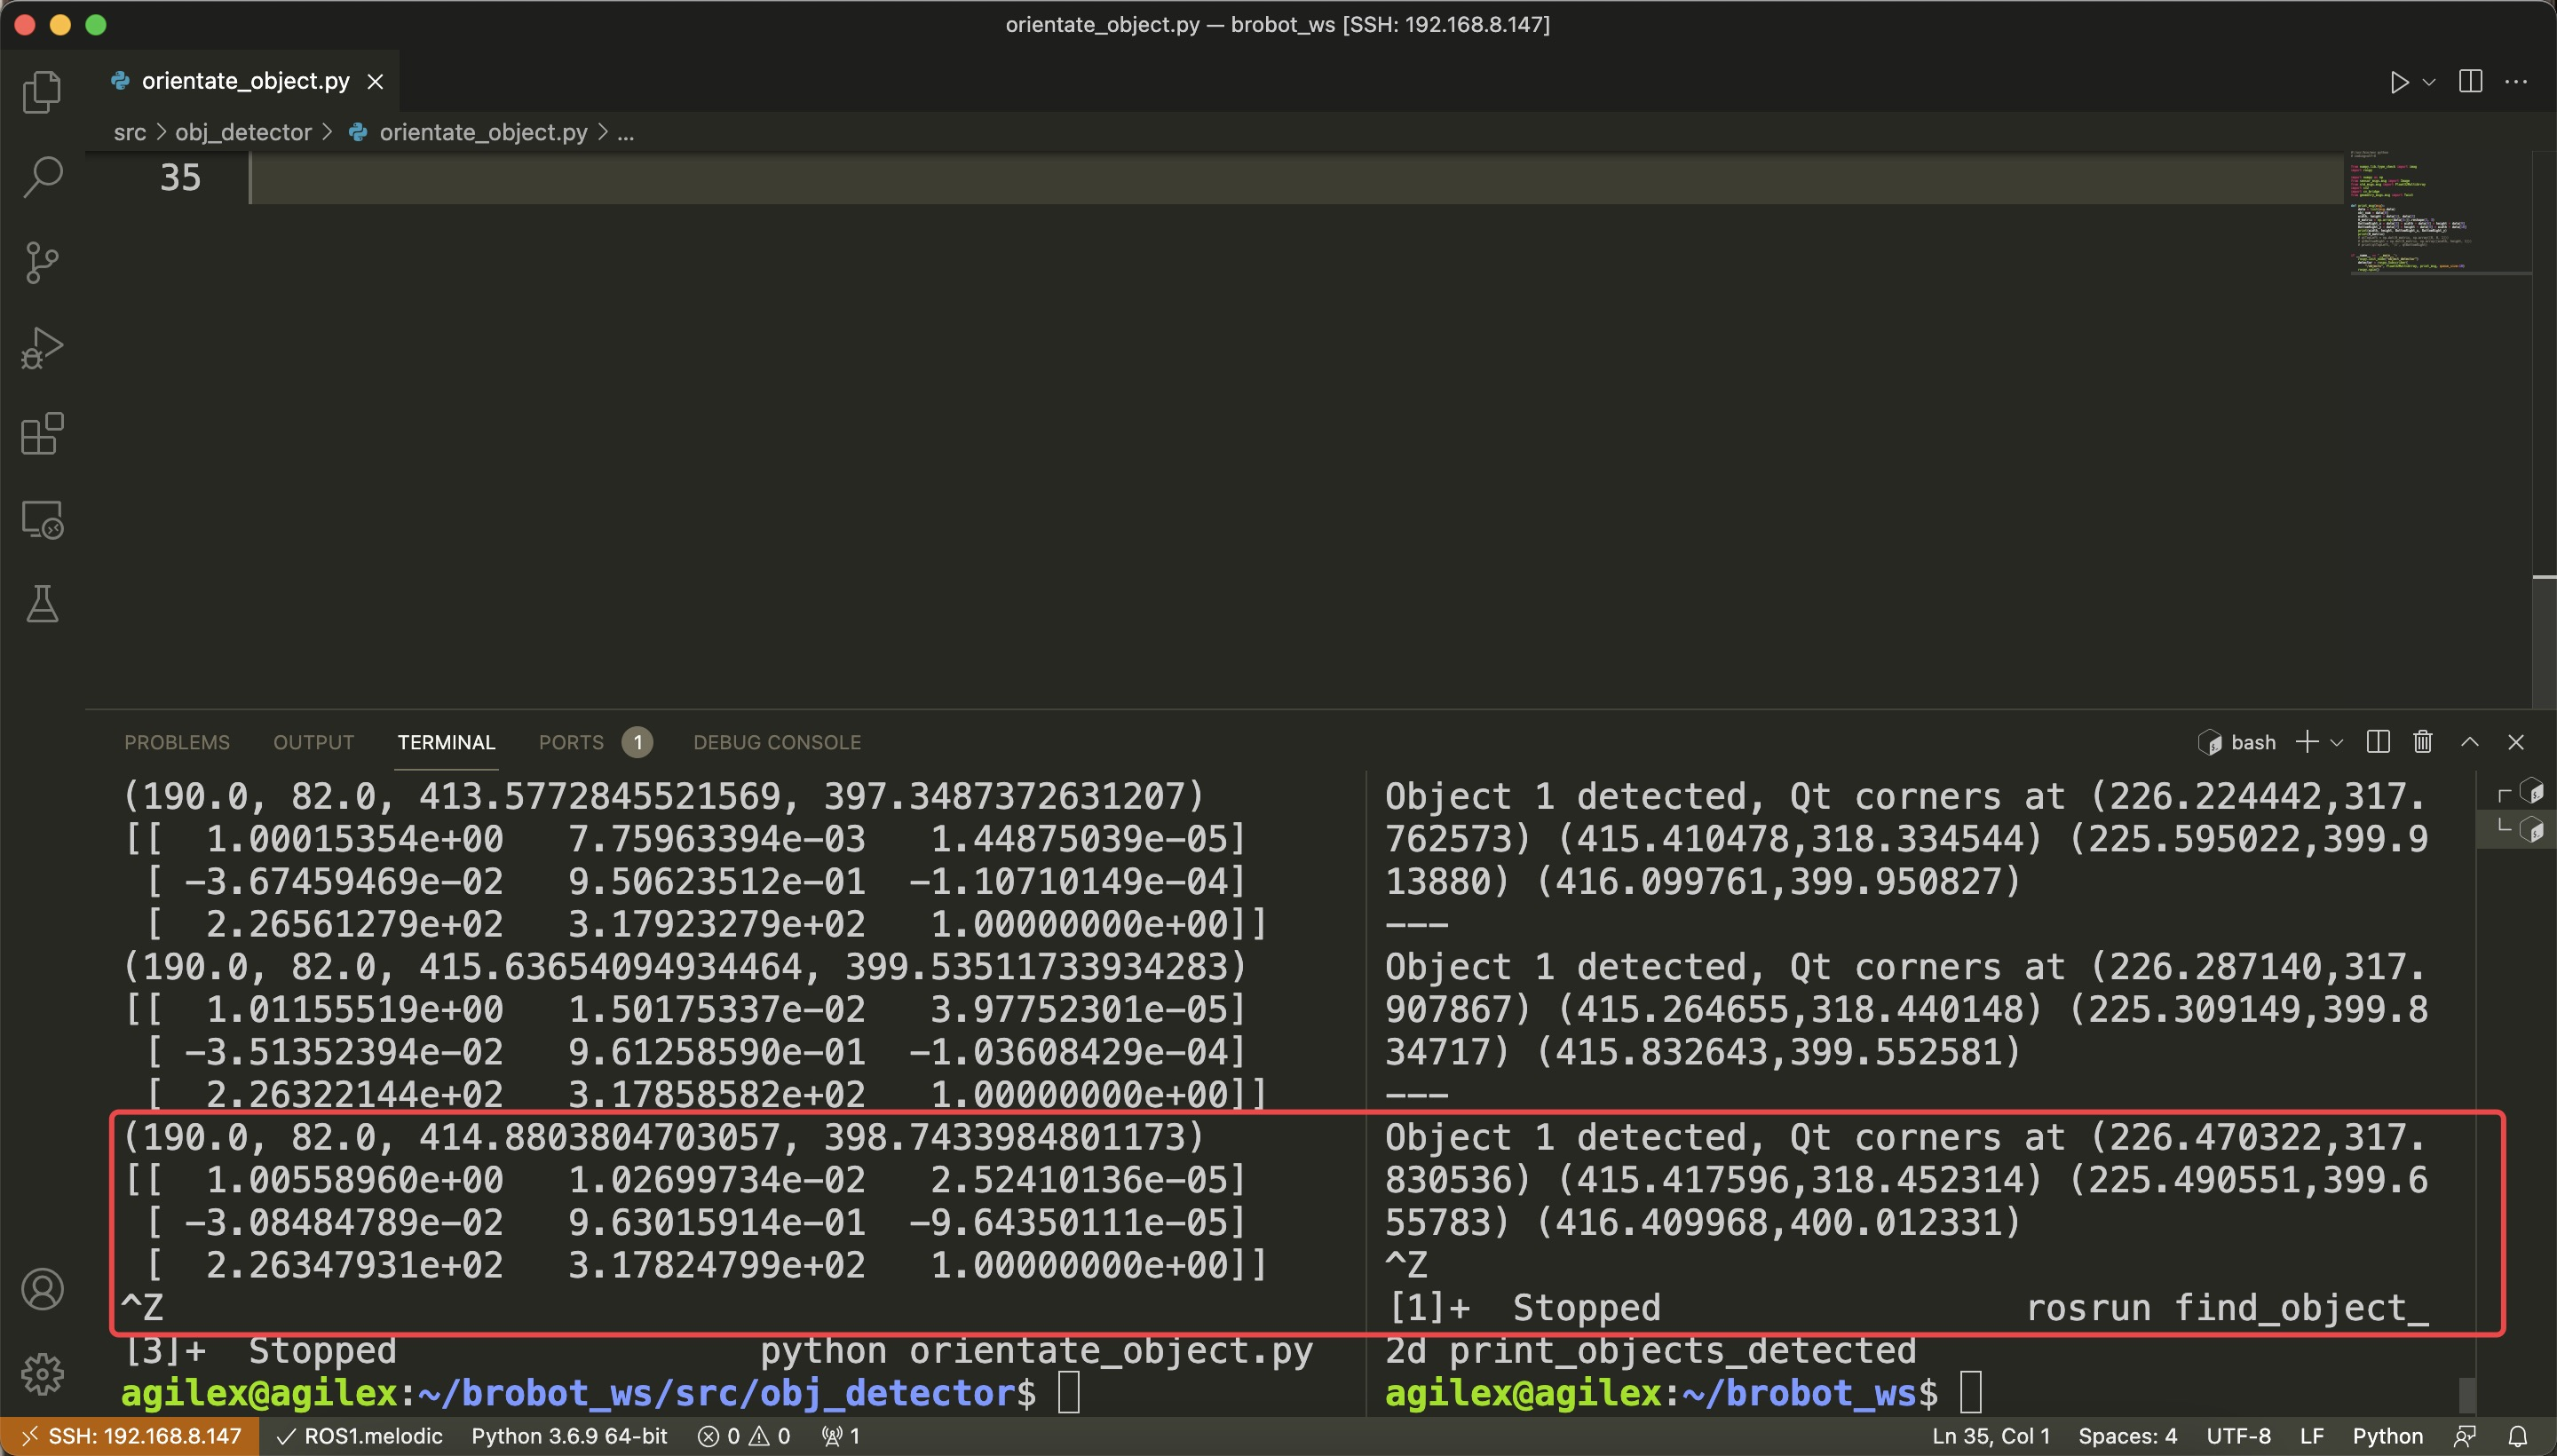
\includegraphics[width=1\linewidth]{findobjectpos.jpg}
		\caption{计算物体的具体位置}
	\end{minipage}
\end{figure}

\subsection{Yolov3-Tiny神经网络训练}
\paragraph{数据集准备}
通过google云端硬盘导入images、ImageSets、annoutations文件夹到darknet文件夹下。
images是图片集合,ImageSets里面有一个次级文件夹:Main,Main里有三个空文件train,test,trainval,val,
annoutations是刚通过精灵标注助手打完且未变成voc所需的标签。并且通过代码将annotation的xml文件转化为voc需要的模式。
\paragraph{配置训练前的参数}
对训练集和测试集图片进行随机划分,并将路径写入四个txt文件中,形成了txt列表。并且生成对应的label文件。之后要修改cfg文件
\begin{enumerate}
	\item 修改cfg文件夹,创建.data和.names文件
	\item .names文件中写入各个类型(要按之前标注标签时的类型顺序额写),这里只有bear一类,因此只写入bear
	      .data文件中写入train valid names文件所在的位置,且需要修改classes(类别数)的参数。
	\item yolo-tiny-vision\_bear.cfg\_train中,将net修改为train模式,把步长设为2000,
	      lr设为0.001.且将classes和filters进行修改,classes修改为1,filters修改为(classes+5)*3。
	      yolo-tiny-vision\_bear.cfg\_test中,只需把.cfg\_train中的Testing部分取消注释,Training部分注释即可。
	\item 将.data文件,.names文件移入Vision\_bear文件下
\end{enumerate}
\paragraph{训练}
先下载预训练模型,之后只需要调用对应的训练命令即可。即训练是对于原有模型的微调。在训练之后我们会使用我们的测试图片进行测试。
从我们的实验结果可以看出我们训练的网络识别准确率还是很高的。

\begin{lstlisting}[caption={模型测试输出}]
[yolo] params: iou loss: mse (2), iou_norm: 0.75, obj_norm: 1.00, cls_norm: 1.00, 
delta_norm: 1.00, scale_x_y: 1.00
Total BFLOPS 5.448 
avg_outputs = 324846 
Allocate additional workspace_size = 52.44 MB 
Loading weights from /content/drive/MyDrive/Vision_bear/yolov3-tiny-Vision_bear_2000.weights...
seen 64, trained: 128 K-images (2 Kilo-batches_64) 
Done! Loaded 24 layers from weights-file 
Detection layer: 16 - type = 28 
Detection layer: 23 - type = 28 
/content/drive/MyDrive/Vision_bear/darknet/images/000056.jpg: Predicted in 4.850000 milli-seconds.
bear: 93%
\end{lstlisting}
\begin{figure}[htbp]
	\begin{center}
		\includegraphics*[width=0.6\linewidth]{yolotest.png}
		\caption{模型测试的图片输出}
	\end{center}
\end{figure}
\paragraph*{}其他具体的代码已经在分享链接中给出 \footnote{https://drive.google.com/file/d/1YCLXn2tdLbZ4lEXn0jRRH7mI\_b9Qm38Z/view?usp=sharing} 。

\subsection{抓取模块}
抓取模块主要是调取给定软件包中的接口(Brobot\_SDK)\upcite{document}。在我们靠近小熊之后,系统会自动启动在机械臂上面的摄像头,并且计算接收到的画面中
小熊物体的中心。这个中心就是机械臂需要达到并且抓取的坐标。在接受坐标之后,机器人只需要调用linear\_movement()函数进行运动即可。
\subsection{模块整合后实验结果}
整合后的实验流程框架就是在附录中给到的流程框图(图片\ref*{task2frame})。

在本次实验中,我们把已有的流程拼接起来,就形成了整个的寻物的任务流程。我们在本次寻物任务中。先进行了巡线行走的任务,
然后开始打开寻物所需要的服务节点,有:机械臂节点、前置摄像头视觉节点、底盘节点、雷达节点、地图服务节点。都打开之后就可以通过
既定的程序进行运行了。

在整个实验中,我们在第19秒完成了巡线任务。此时,我们的程序调用了底层的shell,开启了其他节点的服务。在第50秒的时候,我们的
所有服务都开始运行,小车开始遍历所有规定好的所有节点。在小车巡航到第三个地图的标定的节点的时候(1分44秒),视觉模块发现了小熊的存在。
自此,小车程序将剩余的巡航节点任务都关掉了,开始进行靠近的任务。这个地方我们发现了一个问题就是靠近的时候,小车的速度可以调整的更快
一些,这样可以减少我们在整个任务中所花费的时间。

在2分25秒的时候,我们的小车开始尝试抓取小熊,但是很可惜,因为机械臂标定的问题,我们的机械臂前爪都没有碰到小熊,在平常的实验中是可以
抓起来的,究其原因是因为上次标定太长时间了,太长的时间间隔让机械臂丢失了精度。之后从2分40秒开始我们的小车开始执行回到起点的操作。
在返回起点的过程中我们也卡壳了,因为对于碰撞的容忍度调整的有点低,所以中间在门柱的时候被卡住了一段时间。索性最后还是完成了,虽然存在一些失误
,但是也算是比较成功的实验。

\begin{figure}[htbp]
	\centering
	\begin{minipage}{0.49\linewidth}
		\centering
		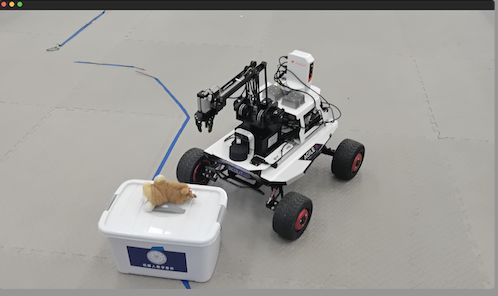
\includegraphics[width=1.0\linewidth]{video1.png}
		\caption{小车尝试抓取}
	\end{minipage}
	%\qquad
	\begin{minipage}{0.49\linewidth}
		\centering
		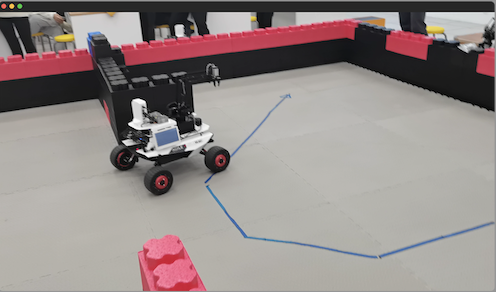
\includegraphics[width=1.0\linewidth]{video2.png}
		\caption{小车回到出发点}
	\end{minipage}
\end{figure}

关键部分具体代码详见附录。

\newpage
\section{出现的问题以及解决方案}
\subsection{硬件问题}
\begin{enumerate}
	\item
	      \textbf{问题:}车载路由器因为接触不良经常出现断连、没有5Gwifi信号、信号质量不好的问题。因此No Machine并不能很好的链接机器人(因为No Machine)
	      需要传输画面信息。

	      \textbf{解决方法:}后面我尝试使用vscode进行链接,vscode不仅有很好的ROS 2扩展支持,而且还可以很清晰地展示文件架构,也可以在
	      vscode上面控制终端的操作。\upcite{roswithvsc}
	\item \textbf{问题:}机械臂经常失去刚性,导致机械臂无法正常响应控制信号。

	      \textbf{解决方法:}在每一次开机的之前,先将机械臂摆正到正确的初始化为止,再开机。这样机械臂的控制器就会
	      在机械臂初始化的时候给予机械臂一定的刚性,并且机械臂可以正确响应。如果以上的操作无法解决机械臂的问题
	      那就将机械臂从机器人上面写下来,重新进行标定,标定后机械臂即可恢复原状。
\end{enumerate}
\subsection{软件问题}
\begin{enumerate}
	\item \textbf{问题:}开启过多的服务时,内存不够用,处理机资源不够用,可能导致一些程序出现致命错误,操作系统可能卡到崩溃。

	      \textbf{解决方法:}后台存在着五个主要的进程,分别是Ros-core, Map-server, Yolov3-tiny, Radar, Movement-Base。
	      在这些进程中,Yolov3-tiny需要的资源是最多的。所以可以给出两种解决方法:
	      \begin{enumerate}
		      \item 增大系统swap分区的大小,让更多不需要系统资源的程序交换到系统的硬盘的虚拟内存空间去。
		      \item 尽量减少神经网络的使用,比如我们可以在检测到黄色色块之后再开启神经网络,让神经网络检测我们看到的是不是小熊。
	      \end{enumerate}
	\item \textbf{问题:} 因为完成整个的任务需要开启过多的服务进程,但是中途又不可以使用鼠标键盘进行操作,找不到一种方法来控制各个进程的启动与关闭。

	      \textbf{解决方法:}使用Python进行进程的控制。使用Python的os库\upcite{ospackage},调用系统shell接口,利用shell开启其他的服务程序,并且记录返回的进程ID号
	      在后面我们会用这些ID号来关闭某些进程,以节约系统资源。比如:我们在抓取任务完成之后,根据神经网络和视觉节点的Process ID关闭他们对应的进程。
\end{enumerate}

\subsection{网络问题}
\begin{enumerate}
	\item \textbf{问题:}有的时候,我们的组上课的时候会到的比较晚,但是实验室内的WiFi带宽有限,甚至链接同一个wifi人多的时候会出现掉线的现象。所以有的时候会出现机器人无法连接到网络的问题。

	      \textbf{解决方法:}一方面是可以开启手机热点,另一方面是可以早点去,连接到别的教室的wifi,别的教室的wifi信号相对较好,而且使用的人也比较少。
	\item \textbf{问题:}下载某些软件包的时候需要访问国外的一些网站,比如www.github.com, wiki.ros.org等等,就会出现无法连接掉线的现象。

	      \textbf{解决方法:}一方面我们小组使用清华等镜像软件站,通过访问国内网站下载相同版本的软件。另一方面我们学习了科学上网的方法,可以访问国外部分的网站学习和下载软件。
\end{enumerate}

\newpage
\section{课程体会}
在本次课程中,我们学习了基本的机器人的编程方法。通过两个课题实践学习到了如何统筹设计机器人控制框架。而且在课题二中我们学习了多个模块:Map\_server, Move\_base, Radar, SLAM等等。
我们先对这些模块分别进行编程实践,对模块的功能有了感性的认识。之后将模块糅合起来,组成了一个适合课题目标的小机器人。

其实我一开始小看了这个课程设计,感觉这个项目应该是很快就可以完成的,但是做到后面发现并不是那么简单。想要一键解决所有问题实在是太难了,不仅是编程的问题,而且还涉及了性能优化,
语言特性,库函数调用,CMake等等问题。一些问题是我曾经没有遇到过的。只能是在实践中学习,摸索着石头过河。在这门课的前面四周,我上课的目标是完成文档中给定的任务就好,但是到了后面
我发现仅仅使用上课的知识并不可以完全解决我。于是我开始寻找网上的学习资料。在YouTube上找到了一个教程\footnote{https://www.youtube.com/watch?v=0aPbWsyENA8\&list=PLLSegLrePWgJudpPUof4-nVFHGkB62Izy},是相当好的。
同时可以多阅读一下文档,比如上面提到的wiki.ros.org,里面提供了很多API的具体调用方法和用途。

到了后面几周,基本就都扑在这个课程设计上面了,基本周末都回去实验室泡着调试机器人,也和很多别的组的大佬一起研究怎么可以把机器人跑起来。第一版的代码也就是这么产生的。
当时也搜了很多网上的代码仓库想看看有没有借鉴的,结果还是没有。中间遇到了很多问题,一开始遇到了小机器人无法定位自我位姿的问题,后面是使用了global\_localization的函数解决的,
在后面考虑要从一个主进程作为入口,开启其他进程。这个使用的python的os库解决的。还学会了如何解决CMake的报错,以及如何安排CMake。还解决了很多其他的问题,就不一一细说了。
但是从这些解决问题的过程中我学到了很多。比如如何高效地利用搜索引擎,如何优雅的使用ROS2自带的文档等等。当然也学到了很多编码方面的能力,比如如何组织大型的工程文件,
如何进行代码的版本管理等等。

最后,很感谢系里可以开这样的一门课程,作为为数不多的工程实践课,感觉学到的东西远比其他理论课学到的东西要更加生动,更加扎实。

\newpage
\appendix
\section{附录}
\subsection{图表}
\begin{figure}[htbp]
	\begin{center}
		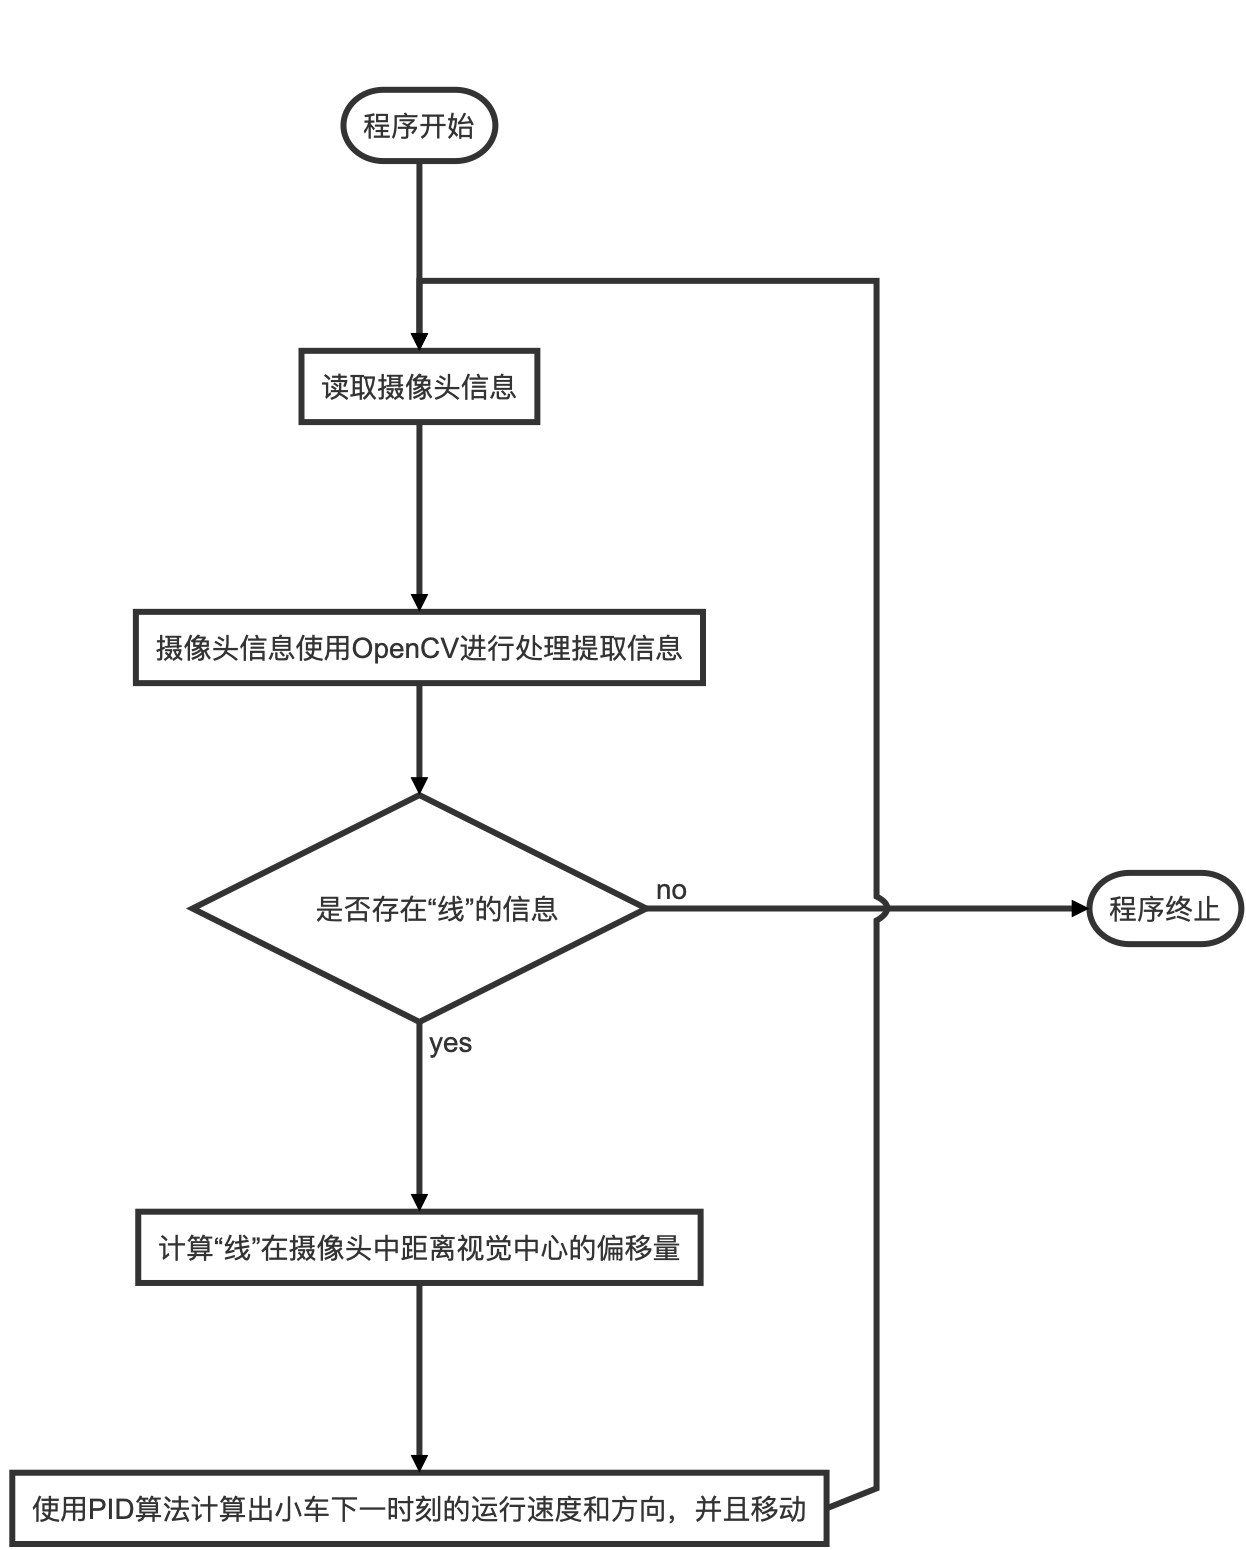
\includegraphics[width=14.5cm]{task1framework.png}
		\caption{task1:巡线框架}
		\label{task1frame}
	\end{center}
\end{figure}
\begin{figure}[htbp]
	\begin{center}
		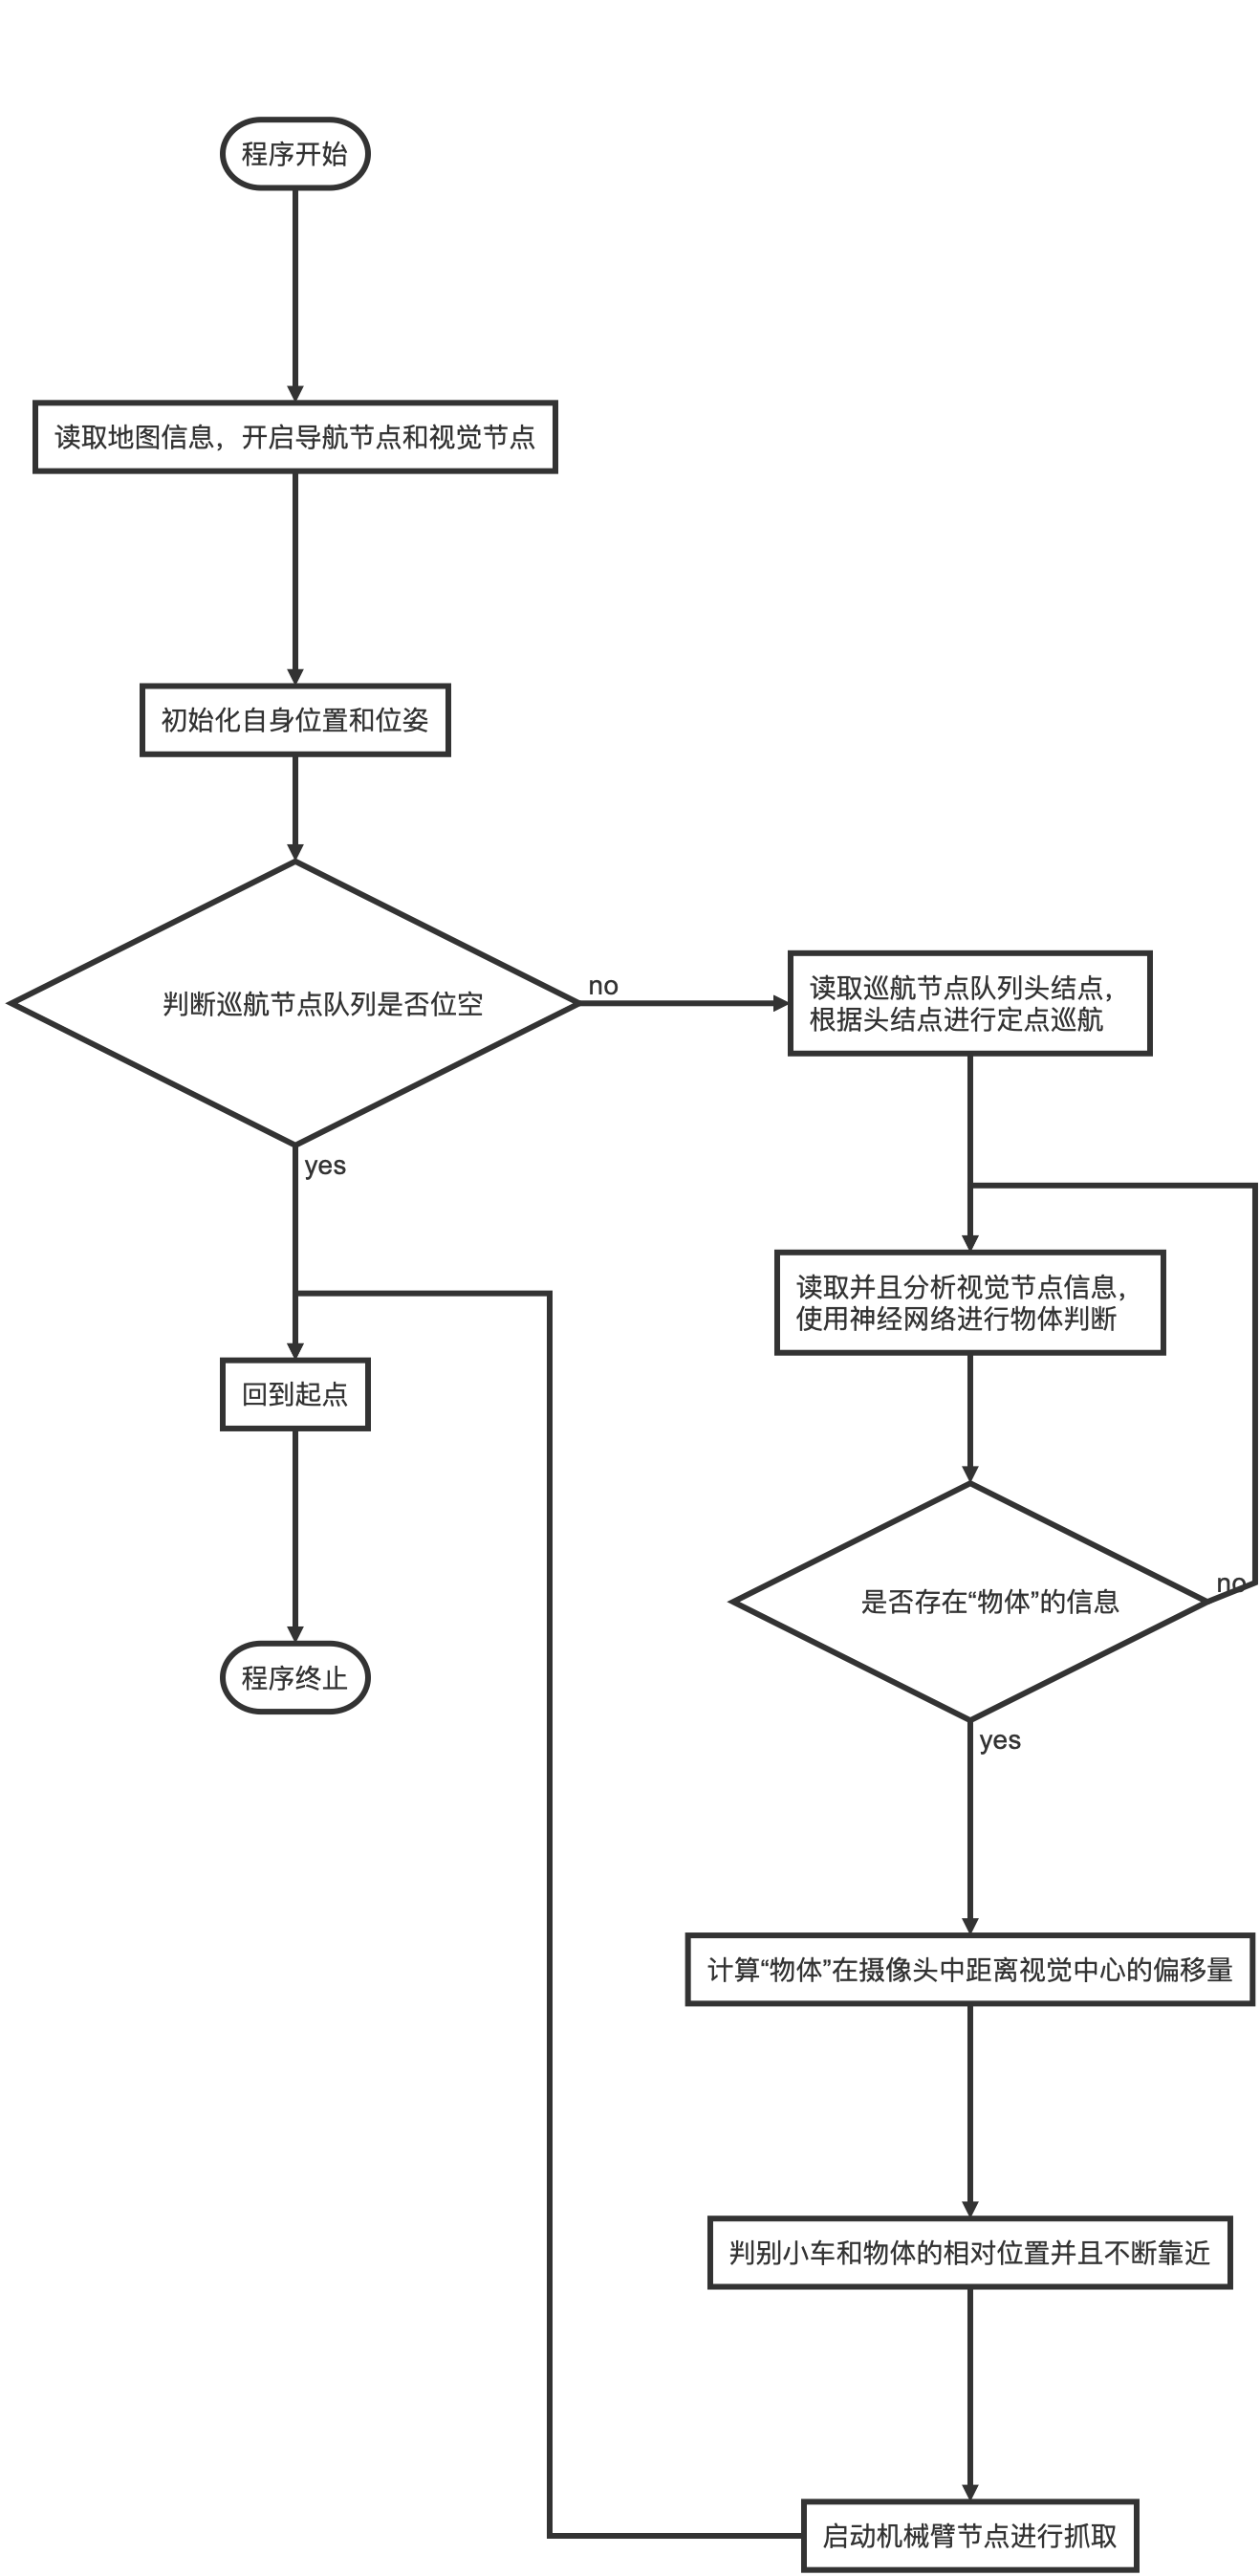
\includegraphics[width=11cm]{task2framework.png}
		\caption{task2:寻物框架}
		\label{task2frame}
	\end{center}
\end{figure}

\newpage
\subsection{Task1--巡线关键代码}
\begin{lstlisting}[language=python, title=巡线关键代码]
def image_callback(self, msg):
        global last_erro, col_black = (73,43,46,124,255,255)# 蓝色的相反色调
        image = self.bridge.imgmsg_to_cv2(msg, desired_encoding='bgr8')
        image = cv2.resize(image, (320,240), interpolation=cv2.INTER_AREA)#提高帧率
        hsv = cv2.cvtColor(image, cv2.COLOR_BGR2HSV) # 转化为HSV
        kernel = numpy.ones((5,5),numpy.uint8)
        hsv_erode = cv2.erode(hsv,kernel,iterations=1)
        hsv_dilate = cv2.dilate(hsv_erode,kernel,iterations=1)
        lowerbH,lowerbS,lowerbV=col_black[0],col_black[1],col_black[2]
        upperbH,upperbS,upperbV=col_black[3],col_black[4],col_black[5]
        mask=cv2.inRange(hsv_dilate,(lowerbH,lowerbS,lowerbV),(upperbH,upperbS,upperbV))
        masked = cv2.bitwise_and(image, image, mask=mask)
        # 在图像某处绘制一个指示,因为只考虑20行宽的图像,所以使用切片将以外的空间区域清空
        h, w, d = image.shape  
        search_bot = search_top = h
        mask[0:search_top, 0:w] = 0
        mask[search_bot:h, 0:w] = 0
        M = cv2.moments(mask) # 计算mask图像的重心,即几何中心
        if M['m00'] > 0:
            cx = int(M['m10']/M['m00'])
            cy = int(M['m01']/M['m00'])
            cv2.circle(image, (cx, cy), 10, (255, 0, 255), -1)
            if cv2.circle:	# 计算图像中心线和目标指示线中心的距离
                erro = cx - w/2-15
                d_erro=erro-last_erro# 计算误差
                self.twist.linear.x = 0.18 
                if erro!=0: self.twist.angular.z = -float(erro)*0.004-float(d_erro)*0.000 #转弯
                else : self.twist.angular.z = 0 # 不转弯
                last_erro=erro
        else:
            self.twist.linear.x = 0
            self.twist.angular.z = 0
            rospy.signal_shutdown("closed!")
        self.cmd_vel_pub.publish(self.twist)
\end{lstlisting}
\newpage
\subsection{Task2--寻物关键代码}
\begin{lstlisting}[language=python, caption=基本巡航框架]
def goal_pose(pose):  # <2>
goal_pose = MoveBaseGoal()
temp = tuple(quaternion_from_euler(0, 0, np.deg2rad(pose[3])))
goal_pose.target_pose.header.frame_id = 'map'
goal_pose.target_pose.pose.position.x = pose[0]
goal_pose.target_pose.pose.position.y = pose[1]
goal_pose.target_pose.pose.position.z = pose[2]
goal_pose.target_pose.pose.orientation.x = temp[0]
goal_pose.target_pose.pose.orientation.y = temp[1]
goal_pose.target_pose.pose.orientation.z = temp[2]
goal_pose.target_pose.pose.orientation.w = temp[3]
return goal_pose

Flag = 0
rospy.init_node('patrol')
client = actionlib.SimpleActionClient('move_base', MoveBaseAction)  # <3>
client.wait_for_server()

def dector_call_back():
global client
print("call_back entered.")
x, y, w, h, area = xywhs[0]
if area > 0.0:
	print("detected.")
	client.cancel_goal()
	client.cancel_all_goals()
	os.chdir('/home/agilex/zycatkin_ws') 
	open_all_subprocess_in_one_go('/home/agilex/zycatkin_ws')
	rospy.signal_shutdown("stop going around!")
else:
	print("no detected.")

if __name__ == '__main__':
cmd_vel_pub = rospy.Publisher("cmd_vel", Twist, queue_size=1)
twist = Twist()
f = Follower()
client.send_goal(goal_pose(waypoints[0]))
while True:
	dector_call_back()
	for pose in waypoints[1:]:   # <4>
		print("goal:x=%f y=%f" % (pose[0], pose[1]))
		goal = goal_pose(pose)
	state = client.get_state()
	while state != GoalStatus.SUCCEEDED:
			state = client.get_state()
	if state == GoalStatus.SUCCEEDED:
			print("reached!")
			client.send_goal(goal)
	print(client.get_result())
	rospy.sleep(1)
\end{lstlisting}

\newpage
\begin{lstlisting}[language=python, caption=位置重定位代码]
	
class localize():
def __init__(self):
	self.pub = rospy.Publisher('/cmd_vel', Twist, queue_size=1)
	self.sub = rospy.Subscriber(
		'/amcl_pose', PoseWithCovarianceStamped, self.callback)
	self.move = Twist()
	self.cov = PoseWithCovarianceStamped()
	rospy.sleep(1)

def serv_client(self):
	wait = rospy.wait_for_service('/global_localization')
	serv_clie = rospy.ServiceProxy('/global_localization', Empty)
	req = EmptyRequest()
	result = serv_clie(req)

def sqr_mov(self):
	self.serv_client()
	rospy.sleep(1)
	print(self.cov.pose.pose.position)
	z = (self.cov.pose.covariance[0] +
		 self.cov.pose.covariance[7] + self.cov.pose.covariance[-1])
	print('cov', z)
	count = 8
	while count > 0:
		self.move_straight()
		rospy.sleep(0.1)
		self.rotate()
		rospy.sleep(0.1)
		count -= 1
		z = (self.cov.pose.covariance[0] + self.cov.pose.covariance[7]\
		+ self.cov.pose.covariance[-1])
		print(self.cov.pose.pose.position)
		print('cov2', z)
	if z < COV_THRESHOLD:
		print('Robot localized itself')
		print('final position', self.cov.pose.pose.position)
	else:
		self.sqr_mov()

def move_straight(self):
	count = 35
	while count > 0:
		self.move.linear.x = 0.15
		self.move.angular.z = 0
		self.pub.publish(self.move)
		rospy.sleep(0.1)
		count -= 1

def rotate(self):
	count = 26
	while count > 0:
		self.move.linear.x = 0.1
		self.move.angular.z = 0.75
		self.pub.publish(self.move)
		rospy.sleep(0.1)
		count -= 1

def callback(self, msg):
	self.cov = msg
	return self.cov

if __name__ == "__main__":
	rospy.init_node('husky_square')
	x = localize()
	x.sqr_mov()
\end{lstlisting}
\newpage
\begin{lstlisting}[language=python, caption=向着物体的方向靠近]
class Detector:
def __init__(self):
	self.detector = rospy.Subscriber(
		"/objects", Float32MultiArray, self.dector_call_back, queue_size=10)
	self.cmd_vel_pub = rospy.Publisher("cmd_vel", Twist, queue_size=1)
	self.twist = Twist()

def fetch_point(self, msg):
	"""
	获取object发布节点返回的数据并且通过坐标变换转化成目标在摄像头中的占比
	image size width = 1280 height = 720
	"""

	def compute_Point(data, x, y):
		"""
		单应矩阵对应坐标点的变换
		"""
		_x = data[3] * x + data[6] * y + data[9]
		_y = data[7] * y + data[4] * x + data[10]
		return (_x, _y)

	def compute_pct(Point):
		return (Point[0] / ImageWidth,  Point[1] / Imageheight)
	# 单应性矩阵求解
	data = list(msg.data)
	obj_num = data[0]
	width, height = data[1], data[2]
	qtTopLeft = compute_Point(data, 0, 0)
	qtTopRight = compute_Point(data, width, 0)
	qtBottomLeft = compute_Point(data, 0, height)
	qtBottomRight = compute_Point(data, width, height)
	return list(map(compute_pct, [qtTopLeft, qtTopRight, qtBottomLeft, qtBottomRight]))

@staticmethod
def compute_center(Points):
	"""
	return cneter_x, center_y
	"""
	point_set = zip(*Points)
	return tuple(map(lambda x: sum(x) / len(x), point_set))

@staticmethod
def compute_coverage(Points):
	x1, y1 = Points[3]
	x2, y2 = Points[0]
	return ((x2-x1)*(y2-y1))

def dector_call_back(self, msg):
	Points = self.fetch_point(msg)
	# print("Points:", Points[0], Points[3])
	center_x, _ = self.compute_center(Points)
	Obj_coverage = self.compute_coverage(Points)
	print("center_x : ", center_x)
	print("Obj_coverage", Obj_coverage)
	Bias = center_x - 0.5
	print("Bias: ", Bias)
	if abs(Bias) > 0.05:
		if Bias > 0:
			print("向右转")
		else:
			print("向左转")
		self.twist.angular.z = -float(Bias) * 0.2
		self.twist.linear.x = 0.05
		self.cmd_vel_pub.publish(self.twist)
	else:
		self.twist.angular.z = 0
		self.twist.linear.x = 0
	self.cmd_vel_pub.publish(self.twist)


if __name__ == '__main__':
rospy.init_node("object_detector")
dector = Detector()
rospy.spin()
\end{lstlisting}
\newpage
\begin{thebibliography}{99}
	\bibitem{rvizvisual} SLAM导航机器人零基础实战系列 https://blog.csdn.net/hiram\_zhang/article/details/88374512
	\bibitem{roswithvsc} 在VScode中配置ROS环境的详细过程 https://www.jb51.net/article/255449.htm
	\bibitem{matrix} 单应性矩阵的求解 https://zhuanlan.zhihu.com/p/163170554
	\bibitem{createdataset} 手把手教你自制VOC,COCO数据集 https://zhuanlan.zhihu.com/p/556197423
	\bibitem{trainyolo} 使用自己的数据训练yolov3-tiny模型 https://blog.csdn.net/fkbiubiubiu/article/details/120295134
	\bibitem{ospackage} Python内置OS库使用文档 https://docs.python.org/3/library/os.html
	\bibitem{document} 复合教育机器人套件用户手册V1.2.pdf
\end{thebibliography}

\end{document}